\lecture{3}{2025-02-24}{Fractional (Nointeger) Number}{}

\section{Fractional number}
\subsection{Fixed-Point Representation}
\begin{parag}{General Format}
    \begin{definition}
        Fixed-Point Numbers are:
        \begin{itemize}
            \item Integers
            \[I = -N, \dots, N\]
            \item Rational numbers ("\textit{binary}" rationals) of the form:
            \[x = \frac{a}{2^f}\]
            where $a \in I$ and $f$ positive integer
        \end{itemize}
    \end{definition}
    The fixed-point representation of a number $x$ consists of integer $x_{int}$ and fraction $x_{fr}$ components represented by $m$ and $f$ digits, respectively:
    \[x = x_{int} + x_{fr}\]
    \begin{definition}
        Digit-vector representation: 
        \[X = (X_{m-1}X_{m-2}\dots X_1X_0\underbrace{.}_{\text{Radix point}}X_{-1}X_{-2}\dots X_{-f})\]
        \begin{itemize}
            \item For \important{unsigned} numbers : 
            \[x = \sum_{i  = -f}^{m-1}X_i2^i\]
            \item For \important{signed} number in two's complement: 
            \[x = -X_{m-1}2^{m-1} + \sum_{i = -f}^{m-2}X_i2^i\]
        \end{itemize}
    \end{definition}
\end{parag}
\subsection{Radix point}
\begin{parag}{Separator between the integer and fractional parts}
    \[X = (X_{m-1}X_{m-2}\dots X_1X_0\underbrace{.}_{\text{Radix point}}X_{-1}X_{-2}\dots X_{-f})\]
    \begin{itemize}
        \item The position of the radix-point is assumed to be fixed
        \begin{itemize}
            \item Hence the name fixed-point
        \end{itemize}
        \item If the radix point is not shown, it is assumed to be to the right of the least significant digit (i.e, no fractional part)
        \begin{itemize}
            \item In that case, the number is an integer
        \end{itemize}
        \item Also known as decimal point, binary point, etc$\dots$
    \end{itemize}
\end{parag}
\begin{center}
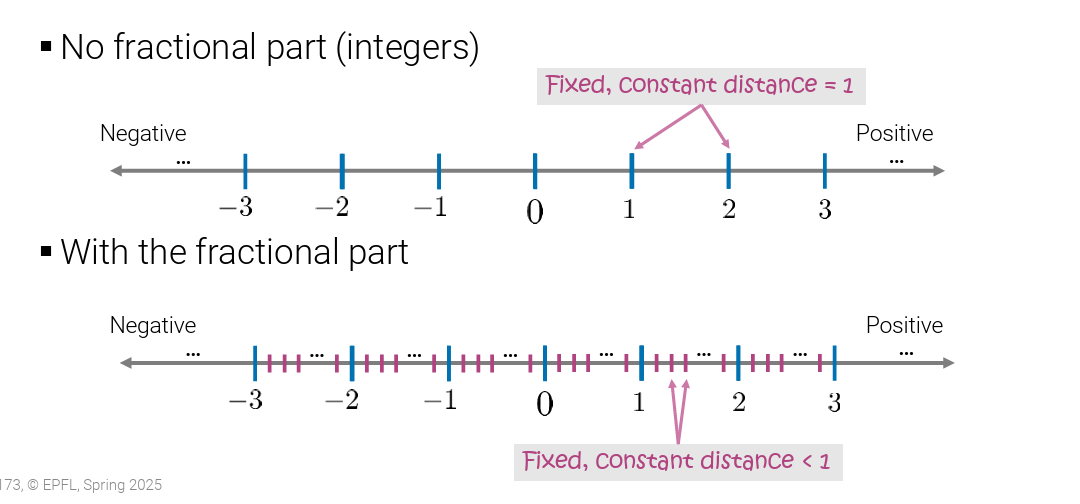
\includegraphics[scale=0.5]{Screenshot 2025-02-24 131346.png}
\end{center}
